%%
%% main.tex
%%
%% Made by
%% Login   <clinares@atlas>
%%
%% Started on  Sat May  4 14:24:58 2019
%% Last update Sat May  4 14:24:58 2019
%%

\documentclass[svgnames,addpoints]{exam}

\usepackage[T1]{fontenc}
\usepackage[utf8]{inputenc}
\usepackage[spanish]{babel}

\usepackage{tb}

\usepackage{amsfonts}
\usepackage{amssymb}
\usepackage{mathtools}

\usepackage{pifont}

\usepackage{cancel}
\usepackage{array}

\usepackage{tikz}
\usepackage{pgflibraryarrows}
\usepackage{pgflibrarysnakes}

\usetikzlibrary{calc,matrix,patterns,fadings,positioning}

\usepackage{xcolor}

\usepackage{array}
\usepackage{eurosym}

\usepackage{booktabs}
\usepackage{url}

\usepackage{rotating}

\newlength{\zerowidth}
\settowidth{\zerowidth}{\huge 0}
\newlength{\zeroheight}
\settoheight{\zeroheight}{\huge 0}

\makeatletter
\def\convertto#1#2{\strip@pt\dimexpr #2*65536/\number\dimexpr 1#1}
\makeatother


\begin{document}

\titulacion{Esquemas}
\asignatura{Secuencias}

\convocatoria{\today}
\tiempo{4 horas}

\begin{tabular}{cc}

  \begin{minipage}{7.5cm}

    \begin{tabular}{c}

      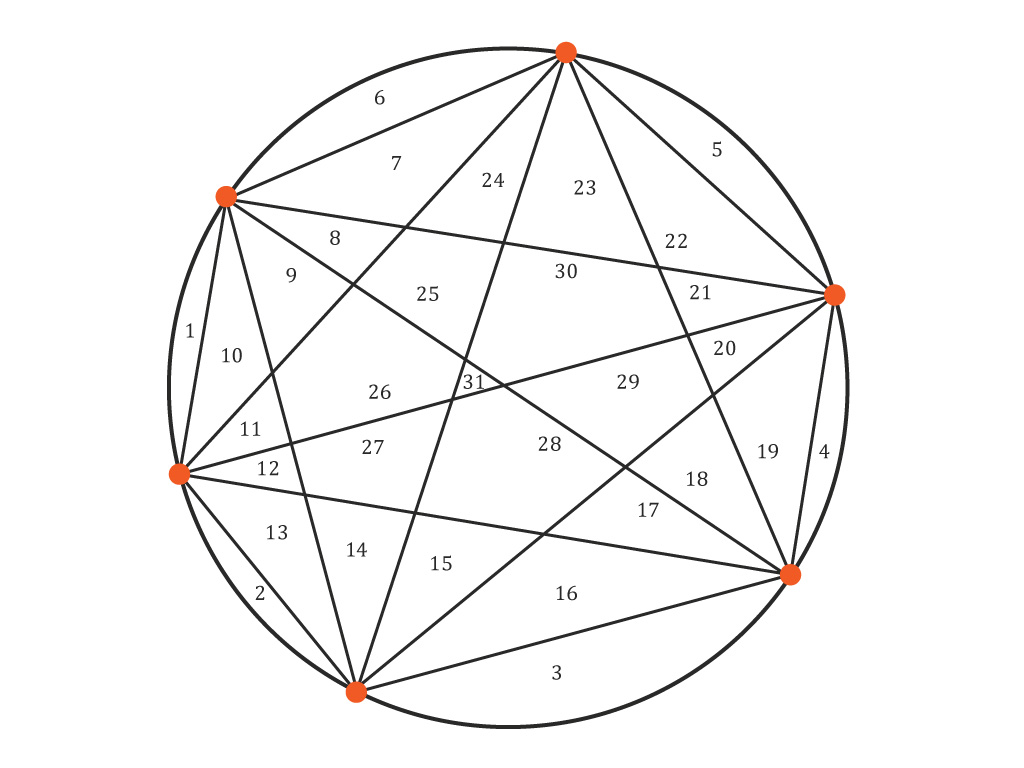
\includegraphics[scale=0.15]{matematica6}\\

    \end{tabular}

  \end{minipage}
  &
  \begin{minipage}{8.5cm}

    \begin{center}

      {\huge \bf \titu}\\
      {\Large \bf \asig}\\ \ \\

      \convo

    \end{center}

  \end{minipage}\\ & \\ & \\  & \\

\end{tabular}

\noindent
{\Large\bf Secuencias}

Todas las representaciones que se muestran a continuación se hacen
empleando las siguientes medidas:

\begin{center}
  \begin{tabular}{ll}
    \texttt{zeroheight}   & \convertto{cm}{\the\zeroheight}\ cm \\
    \texttt{zerowidth}    & \convertto{cm}{\the\zerowidth}\ cm \\
  \end{tabular}
\end{center}

\noindent
y el \texttt{baselineskip} (\convertto{cm}{\the\baselineskip}\
cm). Las dos mostradas arriba deben definirse en el preámbulo del
documento \LaTeX\ (por ejemplo, con un fichero \texttt{.sty} que se
incluya automáticamente en el fichero).

En total, se implementan hasta tres tipos diferentes de secuencias:
\textit{pre}, \textit{post} y \textit{full}. La primera se caracteriza porque se
inicia con un número dado; la segunda tiene el número (o pista) al final; por
último, \textit{full} es un caso de secuencia con al menos una pista y dos
celdas por rellenar donde la pista no está ni al principio ni al final.

\begin{questions}

  \question Primero, se muestran varias secuencias con las siguientes
  características:

  \begin{itemize}

    \item Tipo de secuencia: \textit{pre}

    \item Número maximo de dígitos por celda: 1

    \item Números en la secuencia: 2

  \end{itemize}

  El esquema general se muestra a continuación:

  \noindent\begin{minipage}{0.20\linewidth}
    \begin{center}
      \begin{tikzpicture}

        % --- Coordinates -----------------------------------------------------

        \coordinate (bottom) at (0,0);
        \fill [blue] (bottom) circle (1pt);

        % the first number is located leaving some room to the let so that some
        % sequences can be drawn next to others withouth colliding. For this, 1
        % plus half the number of digits shown in the first number has to be
        % left
        \coordinate (label1) at ($(bottom) + (1.5\zerowidth, 0.5\zeroheight+1.5\baselineskip)$);
        \fill [red] (label1) circle (1pt);

        % the reference point that is located at the center of the answer box
        % should be x-shifted by once the width of zero plus half the width of
        % the answer box, hence 2.5 is multiplied by the width of zero
        \coordinate (answer1) at ($(label1) + (2.5*\zerowidth, 0.0)$);
        \fill [red] (answer1) circle (1pt);

        % ---------------------------------------------------------------------

        % --- Bounding Box ----------------------------------------------------

        % the distance between the answer box and the end of the bounding box is
        % half the width of the bounding box. As this bounding box contains one
        % digit its width is 3.0 and hence 1.5 has to be multiplied by the
        % width of zero
        \coordinate (right) at ($(answer1) + (1.5\zerowidth, 0.5\zeroheight + 0.5\baselineskip)$);
        \fill [green] (right) circle (1pt);

        % draw an invisible box used to properly align all sequences
        \draw [lightgray] (bottom) rectangle (right);

        % ---------------------------------------------------------------------

        % --- Sequence --------------------------------------------------------

        % number
        \draw (label1) node {\huge 4};

        % answer box
        %
        % The width of the answer box is x times the width of zero, where x
        % equals the number of digits to draw plus 2 (to show some slack to the
        % right and left)
        \draw(answer1) node [rounded corners, rectangle, minimum width=3.0*\zerowidth, minimum height = \zeroheight + \baselineskip, draw] {\textcolor{lightgray}{\huge 5}};

        % ---------------------------------------------------------------------

      \end{tikzpicture}
    \end{center}
  \end{minipage}

  A continuación se muestran varios ejemplos con los parámetros anteriores:

  \noindent\begin{minipage}{0.20\linewidth}
    \begin{center}
      \begin{tikzpicture}

        % --- Coordinates -----------------------------------------------------

        \coordinate (bottom) at (0,0);
        \coordinate (label1) at ($(bottom) + (1.5\zerowidth, 0.5\zeroheight+1.5\baselineskip)$);
        \coordinate (answer1) at ($(label1) + (2.5*\zerowidth, 0.0)$);

        % ---------------------------------------------------------------------

        % --- Bounding Box ----------------------------------------------------

        \coordinate (right) at ($(answer1) + (1.5\zerowidth, 0.5\zeroheight + 0.5\baselineskip)$);
        \draw [white] (bottom) rectangle (right);

        % ---------------------------------------------------------------------

        % --- Sequence --------------------------------------------------------

        \draw (label1) node {\huge 4};
        \draw(answer1) node [rounded corners, rectangle, minimum width=3.0*\zerowidth, minimum height = \zeroheight + \baselineskip, draw] {\textcolor{lightgray}{}};

        % ---------------------------------------------------------------------

      \end{tikzpicture}
    \end{center}
  \end{minipage}
  \begin{minipage}{0.20\linewidth}
    \begin{center}
      \begin{tikzpicture}

        % --- Coordinates -----------------------------------------------------

        \coordinate (bottom) at (0,0);
        \coordinate (label1) at ($(bottom) + (1.5\zerowidth, 0.5\zeroheight+1.5\baselineskip)$);
        \coordinate (answer1) at ($(label1) + (2.5*\zerowidth, 0.0)$);

        % ---------------------------------------------------------------------

        % --- Bounding Box ----------------------------------------------------

        \coordinate (right) at ($(answer1) + (1.5\zerowidth, 0.5\zeroheight + 0.5\baselineskip)$);
        \draw [white] (bottom) rectangle (right);

        % ---------------------------------------------------------------------

        % --- Sequence --------------------------------------------------------

        \draw (label1) node {\huge 6};
        \draw(answer1) node [rounded corners, rectangle, minimum width=3.0*\zerowidth, minimum height = \zeroheight + \baselineskip, draw] {\textcolor{lightgray}{}};

        % ---------------------------------------------------------------------

      \end{tikzpicture}
    \end{center}
  \end{minipage}
  \begin{minipage}{0.20\linewidth}
    \begin{center}
      \begin{tikzpicture}

        % --- Coordinates -----------------------------------------------------

        \coordinate (bottom) at (0,0);
        \coordinate (label1) at ($(bottom) + (1.5\zerowidth, 0.5\zeroheight+1.5\baselineskip)$);
        \coordinate (answer1) at ($(label1) + (2.5*\zerowidth, 0.0)$);

        % ---------------------------------------------------------------------

        % --- Bounding Box ----------------------------------------------------

        \coordinate (right) at ($(answer1) + (1.5\zerowidth, 0.5\zeroheight + 0.5\baselineskip)$);
        \draw [white] (bottom) rectangle (right);

        % ---------------------------------------------------------------------

        % --- Sequence --------------------------------------------------------

        \draw (label1) node {\huge 2};
        \draw(answer1) node [rounded corners, rectangle, minimum width=3.0*\zerowidth, minimum height = \zeroheight + \baselineskip, draw] {\textcolor{lightgray}{}};

        % ---------------------------------------------------------------------

      \end{tikzpicture}
    \end{center}
  \end{minipage}
  \begin{minipage}{0.20\linewidth}
    \begin{center}
      \begin{tikzpicture}

        % --- Coordinates -----------------------------------------------------

        \coordinate (bottom) at (0,0);
        \coordinate (label1) at ($(bottom) + (1.5\zerowidth, 0.5\zeroheight+1.5\baselineskip)$);
        \coordinate (answer1) at ($(label1) + (2.5*\zerowidth, 0.0)$);

        % ---------------------------------------------------------------------

        % --- Bounding Box ----------------------------------------------------

        \coordinate (right) at ($(answer1) + (1.5\zerowidth, 0.5\zeroheight + 0.5\baselineskip)$);
        \draw [white] (bottom) rectangle (right);

        % ---------------------------------------------------------------------

        % --- Sequence --------------------------------------------------------

        \draw (label1) node {\huge 8};
        \draw(answer1) node [rounded corners, rectangle, minimum width=3.0*\zerowidth, minimum height = \zeroheight + \baselineskip, draw] {\textcolor{lightgray}{}};

        % ---------------------------------------------------------------------

      \end{tikzpicture}
    \end{center}
  \end{minipage}
\begin{minipage}{0.20\linewidth}
    \begin{center}
      \begin{tikzpicture}

        % --- Coordinates -----------------------------------------------------

        \coordinate (bottom) at (0,0);
        \coordinate (label1) at ($(bottom) + (1.5\zerowidth, 0.5\zeroheight+1.5\baselineskip)$);
        \coordinate (answer1) at ($(label1) + (2.5*\zerowidth, 0.0)$);

        % ---------------------------------------------------------------------

        % --- Bounding Box ----------------------------------------------------

        \coordinate (right) at ($(answer1) + (1.5\zerowidth, 0.5\zeroheight + 0.5\baselineskip)$);
        \draw [white] (bottom) rectangle (right);

        % ---------------------------------------------------------------------

        % --- Sequence --------------------------------------------------------

        \draw (label1) node {\huge 3};
        \draw(answer1) node [rounded corners, rectangle, minimum width=3.0*\zerowidth, minimum height = \zeroheight + \baselineskip, draw] {\textcolor{lightgray}{}};

        % ---------------------------------------------------------------------

      \end{tikzpicture}
    \end{center}
  \end{minipage}
  \begin{minipage}{0.20\linewidth}
    \begin{center}
      \begin{tikzpicture}

        % --- Coordinates -----------------------------------------------------

        \coordinate (bottom) at (0,0);
        \coordinate (label1) at ($(bottom) + (1.5\zerowidth, 0.5\zeroheight+1.5\baselineskip)$);
        \coordinate (answer1) at ($(label1) + (2.5*\zerowidth, 0.0)$);

        % ---------------------------------------------------------------------

        % --- Bounding Box ----------------------------------------------------

        \coordinate (right) at ($(answer1) + (1.5\zerowidth, 0.5\zeroheight + 0.5\baselineskip)$);
        \draw [white] (bottom) rectangle (right);

        % ---------------------------------------------------------------------

        % --- Sequence --------------------------------------------------------

        \draw (label1) node {\huge 5};
        \draw(answer1) node [rounded corners, rectangle, minimum width=3.0*\zerowidth, minimum height = \zeroheight + \baselineskip, draw] {\textcolor{lightgray}{}};

        % ---------------------------------------------------------------------

      \end{tikzpicture}
    \end{center}
  \end{minipage}
  \begin{minipage}{0.20\linewidth}
    \begin{center}
      \begin{tikzpicture}

        % --- Coordinates -----------------------------------------------------

        \coordinate (bottom) at (0,0);
        \coordinate (label1) at ($(bottom) + (1.5\zerowidth, 0.5\zeroheight+1.5\baselineskip)$);
        \coordinate (answer1) at ($(label1) + (2.5*\zerowidth, 0.0)$);

        % ---------------------------------------------------------------------

        % --- Bounding Box ----------------------------------------------------

        \coordinate (right) at ($(answer1) + (1.5\zerowidth, 0.5\zeroheight + 0.5\baselineskip)$);
        \draw [white] (bottom) rectangle (right);

        % ---------------------------------------------------------------------

        % --- Sequence --------------------------------------------------------

        \draw (label1) node {\huge 0};
        \draw(answer1) node [rounded corners, rectangle, minimum width=3.0*\zerowidth, minimum height = \zeroheight + \baselineskip, draw] {\textcolor{lightgray}{}};

        % ---------------------------------------------------------------------

      \end{tikzpicture}
    \end{center}
  \end{minipage}
  \begin{minipage}{0.20\linewidth}
    \begin{center}
      \begin{tikzpicture}

        % --- Coordinates -----------------------------------------------------

        \coordinate (bottom) at (0,0);
        \coordinate (label1) at ($(bottom) + (1.5\zerowidth, 0.5\zeroheight+1.5\baselineskip)$);
        \coordinate (answer1) at ($(label1) + (2.5*\zerowidth, 0.0)$);

        % ---------------------------------------------------------------------

        % --- Bounding Box ----------------------------------------------------

        \coordinate (right) at ($(answer1) + (1.5\zerowidth, 0.5\zeroheight + 0.5\baselineskip)$);
        \draw [white] (bottom) rectangle (right);

        % ---------------------------------------------------------------------

        % --- Sequence --------------------------------------------------------

        \draw (label1) node {\huge 1};
        \draw(answer1) node [rounded corners, rectangle, minimum width=3.0*\zerowidth, minimum height = \zeroheight + \baselineskip, draw] {\textcolor{lightgray}{}};

        % ---------------------------------------------------------------------

      \end{tikzpicture}
    \end{center}
  \end{minipage}
  \begin{minipage}{0.20\linewidth}
    \begin{center}
      \begin{tikzpicture}

        % --- Coordinates -----------------------------------------------------

        \coordinate (bottom) at (0,0);
        \coordinate (label1) at ($(bottom) + (1.5\zerowidth, 0.5\zeroheight+1.5\baselineskip)$);
        \coordinate (answer1) at ($(label1) + (2.5*\zerowidth, 0.0)$);

        % ---------------------------------------------------------------------

        % --- Bounding Box ----------------------------------------------------

        \coordinate (right) at ($(answer1) + (1.5\zerowidth, 0.5\zeroheight + 0.5\baselineskip)$);
        \draw [white] (bottom) rectangle (right);

        % ---------------------------------------------------------------------

        % --- Sequence --------------------------------------------------------

        \draw (label1) node {\huge 6};
        \draw(answer1) node [rounded corners, rectangle, minimum width=3.0*\zerowidth, minimum height = \zeroheight + \baselineskip, draw] {\textcolor{lightgray}{}};

        % ---------------------------------------------------------------------

      \end{tikzpicture}
    \end{center}
  \end{minipage}
  \begin{minipage}{0.20\linewidth}
    \begin{center}
      \begin{tikzpicture}

        % --- Coordinates -----------------------------------------------------

        \coordinate (bottom) at (0,0);
        \coordinate (label1) at ($(bottom) + (1.5\zerowidth, 0.5\zeroheight+1.5\baselineskip)$);
        \coordinate (answer1) at ($(label1) + (2.5*\zerowidth, 0.0)$);

        % ---------------------------------------------------------------------

        % --- Bounding Box ----------------------------------------------------

        \coordinate (right) at ($(answer1) + (1.5\zerowidth, 0.5\zeroheight + 0.5\baselineskip)$);
        \draw [white] (bottom) rectangle (right);

        % ---------------------------------------------------------------------

        % --- Sequence --------------------------------------------------------

        \draw (label1) node {\huge 7};
        \draw(answer1) node [rounded corners, rectangle, minimum width=3.0*\zerowidth, minimum height = \zeroheight + \baselineskip, draw] {\textcolor{lightgray}{}};

        % ---------------------------------------------------------------------

      \end{tikzpicture}
    \end{center}
  \end{minipage}

  \question Ahora se muestran varias secuencias con las siguientes
  características:

  \begin{itemize}

    \item Tipo de secuencia: \textit{pre}

    \item Número maximo de dígitos por celda: 2

    \item Números en la secuencia: 2

  \end{itemize}

  El esquema general se muestra a continuación:

  \noindent\begin{minipage}{0.20\linewidth}
    \begin{center}
      \begin{tikzpicture}

        % --- Coordinates -----------------------------------------------------

        \coordinate (bottom) at (0,0);
        \fill [blue] (bottom) circle (1pt);

        % the first number is located leaving some room to the let so that some
        % sequences can be drawn next to others withouth colliding. For this, 1
        % plus half the number of digits shown in the first number has to be
        % left
        \coordinate (label1) at ($(bottom) + (2.0\zerowidth, 0.5\zeroheight+1.5\baselineskip)$);
        \fill [red] (label1) circle (1pt);

        % the reference point that is located at the center of the answer box
        % should be x-shifted by once the width of zero plus half the width of
        % the answer box, this sums up to 2.5 is multiplied by the width of
        % zero. In addition, half the number of digits of the number located at
        % (label1) is added also. In this case, the number consists of two
        % digits and hence 1 is added also, resulting in 3.5
        \coordinate (answer1) at ($(label1) + (3.5*\zerowidth, 0.0)$);
        \fill [red] (answer1) circle (1pt);

        % ---------------------------------------------------------------------

        % --- Bounding Box ----------------------------------------------------

        % the distance between the answer box and the end of the bounding box is
        % half the width of the bounding box. As this bounding box contains two
        % digits its width is 4.0 and hence 2.0 has to be multiplied by the
        % width of zero
        \coordinate (right) at ($(answer1) + (2.0\zerowidth, 0.5\zeroheight + 0.5\baselineskip)$);
        \fill [green] (right) circle (1pt);

        % draw an invisible box used to properly align all sequences
        \draw [lightgray] (bottom) rectangle (right);

        % ---------------------------------------------------------------------

        % --- Sequence --------------------------------------------------------

        % number
        \draw (label1) node {\huge 24};

        % answer box
        %
        % The width of the answer box is x times the width of zero, where x
        % equals the number of digits to draw plus 2 (to show some slack to the
        % right and left)
        \draw(answer1) node [rounded corners, rectangle, minimum width=4.0*\zerowidth, minimum height = \zeroheight + \baselineskip, draw] {\textcolor{lightgray}{\huge 25}};

        % ---------------------------------------------------------------------

      \end{tikzpicture}
    \end{center}
  \end{minipage}

  A continuación se muestran varios ejemplos con los parámetros anteriores:

  \noindent\begin{minipage}{0.20\linewidth}
    \begin{center}
      \begin{tikzpicture}

        % --- Coordinates -----------------------------------------------------

        \coordinate (bottom) at (0,0);
        \coordinate (label1) at ($(bottom) + (1.5\zerowidth, 0.5\zeroheight+1.5\baselineskip)$);
        \coordinate (answer1) at ($(label1) + (3.5*\zerowidth, 0.0)$);

        % ---------------------------------------------------------------------

        % --- Bounding Box ----------------------------------------------------

        \coordinate (right) at ($(answer1) + (2.0\zerowidth, 0.5\zeroheight + 0.5\baselineskip)$);
        \draw [white] (bottom) rectangle (right);

        % ---------------------------------------------------------------------

        % --- Sequence --------------------------------------------------------

        \draw (label1) node {\huge 24};
        \draw(answer1) node [rounded corners, rectangle, minimum width=4.0*\zerowidth, minimum height = \zeroheight + \baselineskip, draw] {\textcolor{lightgray}{}};

        % ---------------------------------------------------------------------

      \end{tikzpicture}
    \end{center}
  \end{minipage}
  \noindent\begin{minipage}{0.20\linewidth}
    \begin{center}
      \begin{tikzpicture}

        % --- Coordinates -----------------------------------------------------

        \coordinate (bottom) at (0,0);
        \coordinate (label1) at ($(bottom) + (1.5\zerowidth, 0.5\zeroheight+1.5\baselineskip)$);
        \coordinate (answer1) at ($(label1) + (3.5*\zerowidth, 0.0)$);

        % ---------------------------------------------------------------------

        % --- Bounding Box ----------------------------------------------------

        \coordinate (right) at ($(answer1) + (2.0\zerowidth, 0.5\zeroheight + 0.5\baselineskip)$);
        \draw [white] (bottom) rectangle (right);

        % ---------------------------------------------------------------------

        % --- Sequence --------------------------------------------------------

        \draw (label1) node {\huge 34};
        \draw(answer1) node [rounded corners, rectangle, minimum width=4.0*\zerowidth, minimum height = \zeroheight + \baselineskip, draw] {\textcolor{lightgray}{}};

        % ---------------------------------------------------------------------

      \end{tikzpicture}
    \end{center}
  \end{minipage}
  \noindent\begin{minipage}{0.20\linewidth}
    \begin{center}
      \begin{tikzpicture}

        % --- Coordinates -----------------------------------------------------

        \coordinate (bottom) at (0,0);
        \coordinate (label1) at ($(bottom) + (1.5\zerowidth, 0.5\zeroheight+1.5\baselineskip)$);
        \coordinate (answer1) at ($(label1) + (3.5*\zerowidth, 0.0)$);

        % ---------------------------------------------------------------------

        % --- Bounding Box ----------------------------------------------------

        \coordinate (right) at ($(answer1) + (2.0\zerowidth, 0.5\zeroheight + 0.5\baselineskip)$);
        \draw [white] (bottom) rectangle (right);

        % ---------------------------------------------------------------------

        % --- Sequence --------------------------------------------------------

        \draw (label1) node {\huge 70};
        \draw(answer1) node [rounded corners, rectangle, minimum width=4.0*\zerowidth, minimum height = \zeroheight + \baselineskip, draw] {\textcolor{lightgray}{}};

        % ---------------------------------------------------------------------

      \end{tikzpicture}
    \end{center}
  \end{minipage}
  \noindent\begin{minipage}{0.20\linewidth}
    \begin{center}
      \begin{tikzpicture}

        % --- Coordinates -----------------------------------------------------

        \coordinate (bottom) at (0,0);
        \coordinate (label1) at ($(bottom) + (1.5\zerowidth, 0.5\zeroheight+1.5\baselineskip)$);
        \coordinate (answer1) at ($(label1) + (3.5*\zerowidth, 0.0)$);

        % ---------------------------------------------------------------------

        % --- Bounding Box ----------------------------------------------------

        \coordinate (right) at ($(answer1) + (2.0\zerowidth, 0.5\zeroheight + 0.5\baselineskip)$);
        \draw [white] (bottom) rectangle (right);

        % ---------------------------------------------------------------------

        % --- Sequence --------------------------------------------------------

        \draw (label1) node {\huge 66};
        \draw(answer1) node [rounded corners, rectangle, minimum width=4.0*\zerowidth, minimum height = \zeroheight + \baselineskip, draw] {\textcolor{lightgray}{}};

        % ---------------------------------------------------------------------

      \end{tikzpicture}
    \end{center}
  \end{minipage}
  \noindent\begin{minipage}{0.20\linewidth}
    \begin{center}
      \begin{tikzpicture}

        % --- Coordinates -----------------------------------------------------

        \coordinate (bottom) at (0,0);
        \coordinate (label1) at ($(bottom) + (1.5\zerowidth, 0.5\zeroheight+1.5\baselineskip)$);
        \coordinate (answer1) at ($(label1) + (3.5*\zerowidth, 0.0)$);

        % ---------------------------------------------------------------------

        % --- Bounding Box ----------------------------------------------------

        \coordinate (right) at ($(answer1) + (2.0\zerowidth, 0.5\zeroheight + 0.5\baselineskip)$);
        \draw [white] (bottom) rectangle (right);

        % ---------------------------------------------------------------------

        % --- Sequence --------------------------------------------------------

        \draw (label1) node {\huge 58};
        \draw(answer1) node [rounded corners, rectangle, minimum width=4.0*\zerowidth, minimum height = \zeroheight + \baselineskip, draw] {\textcolor{lightgray}{}};

        % ---------------------------------------------------------------------

      \end{tikzpicture}
    \end{center}
  \end{minipage}
  \noindent\begin{minipage}{0.20\linewidth}
    \begin{center}
      \begin{tikzpicture}

        % --- Coordinates -----------------------------------------------------

        \coordinate (bottom) at (0,0);
        \coordinate (label1) at ($(bottom) + (1.5\zerowidth, 0.5\zeroheight+1.5\baselineskip)$);
        \coordinate (answer1) at ($(label1) + (3.5*\zerowidth, 0.0)$);

        % ---------------------------------------------------------------------

        % --- Bounding Box ----------------------------------------------------

        \coordinate (right) at ($(answer1) + (2.0\zerowidth, 0.5\zeroheight + 0.5\baselineskip)$);
        \draw [white] (bottom) rectangle (right);

        % ---------------------------------------------------------------------

        % --- Sequence --------------------------------------------------------

        \draw (label1) node {\huge 37};
        \draw(answer1) node [rounded corners, rectangle, minimum width=4.0*\zerowidth, minimum height = \zeroheight + \baselineskip, draw] {\textcolor{lightgray}{}};

        % ---------------------------------------------------------------------

      \end{tikzpicture}
    \end{center}
  \end{minipage}
  \noindent\begin{minipage}{0.20\linewidth}
    \begin{center}
      \begin{tikzpicture}

        % --- Coordinates -----------------------------------------------------

        \coordinate (bottom) at (0,0);
        \coordinate (label1) at ($(bottom) + (1.5\zerowidth, 0.5\zeroheight+1.5\baselineskip)$);
        \coordinate (answer1) at ($(label1) + (3.5*\zerowidth, 0.0)$);

        % ---------------------------------------------------------------------

        % --- Bounding Box ----------------------------------------------------

        \coordinate (right) at ($(answer1) + (2.0\zerowidth, 0.5\zeroheight + 0.5\baselineskip)$);
        \draw [white] (bottom) rectangle (right);

        % ---------------------------------------------------------------------

        % --- Sequence --------------------------------------------------------

        \draw (label1) node {\huge 16};
        \draw(answer1) node [rounded corners, rectangle, minimum width=4.0*\zerowidth, minimum height = \zeroheight + \baselineskip, draw] {\textcolor{lightgray}{}};

        % ---------------------------------------------------------------------

      \end{tikzpicture}
    \end{center}
  \end{minipage}
  \noindent\begin{minipage}{0.20\linewidth}
    \begin{center}
      \begin{tikzpicture}

        % --- Coordinates -----------------------------------------------------

        \coordinate (bottom) at (0,0);
        \coordinate (label1) at ($(bottom) + (1.5\zerowidth, 0.5\zeroheight+1.5\baselineskip)$);
        \coordinate (answer1) at ($(label1) + (3.5*\zerowidth, 0.0)$);

        % ---------------------------------------------------------------------

        % --- Bounding Box ----------------------------------------------------

        \coordinate (right) at ($(answer1) + (2.0\zerowidth, 0.5\zeroheight + 0.5\baselineskip)$);
        \draw [white] (bottom) rectangle (right);

        % ---------------------------------------------------------------------

        % --- Sequence --------------------------------------------------------

        \draw (label1) node {\huge 89};
        \draw(answer1) node [rounded corners, rectangle, minimum width=4.0*\zerowidth, minimum height = \zeroheight + \baselineskip, draw] {\textcolor{lightgray}{}};

        % ---------------------------------------------------------------------

      \end{tikzpicture}
    \end{center}
  \end{minipage}
  \noindent\begin{minipage}{0.20\linewidth}
    \begin{center}
      \begin{tikzpicture}

        % --- Coordinates -----------------------------------------------------

        \coordinate (bottom) at (0,0);
        \coordinate (label1) at ($(bottom) + (1.5\zerowidth, 0.5\zeroheight+1.5\baselineskip)$);
        \coordinate (answer1) at ($(label1) + (3.5*\zerowidth, 0.0)$);

        % ---------------------------------------------------------------------

        % --- Bounding Box ----------------------------------------------------

        \coordinate (right) at ($(answer1) + (2.0\zerowidth, 0.5\zeroheight + 0.5\baselineskip)$);
        \draw [white] (bottom) rectangle (right);

        % ---------------------------------------------------------------------

        % --- Sequence --------------------------------------------------------

        \draw (label1) node {\huge 93};
        \draw(answer1) node [rounded corners, rectangle, minimum width=4.0*\zerowidth, minimum height = \zeroheight + \baselineskip, draw] {\textcolor{lightgray}{}};

        % ---------------------------------------------------------------------

      \end{tikzpicture}
    \end{center}
  \end{minipage}
  \noindent\begin{minipage}{0.20\linewidth}
    \begin{center}
      \begin{tikzpicture}

        % --- Coordinates -----------------------------------------------------

        \coordinate (bottom) at (0,0);
        \coordinate (label1) at ($(bottom) + (1.5\zerowidth, 0.5\zeroheight+1.5\baselineskip)$);
        \coordinate (answer1) at ($(label1) + (3.5*\zerowidth, 0.0)$);

        % ---------------------------------------------------------------------

        % --- Bounding Box ----------------------------------------------------

        \coordinate (right) at ($(answer1) + (2.0\zerowidth, 0.5\zeroheight + 0.5\baselineskip)$);
        \draw [white] (bottom) rectangle (right);

        % ---------------------------------------------------------------------

        % --- Sequence --------------------------------------------------------

        \draw (label1) node {\huge 42};
        \draw(answer1) node [rounded corners, rectangle, minimum width=4.0*\zerowidth, minimum height = \zeroheight + \baselineskip, draw] {\textcolor{lightgray}{}};

        % ---------------------------------------------------------------------

      \end{tikzpicture}
    \end{center}
  \end{minipage}

  \question En tercer lugar, se muestran varias secuencias con las siguientes
  características:

  \begin{itemize}

    \item Tipo de secuencia: \textit{pre}

    \item Número maximo de dígitos por celda: 3

    \item Números en la secuencia: 2

  \end{itemize}

  El esquema general se muestra a continuación:

  \noindent\begin{minipage}{0.20\linewidth}
    \begin{center}
      \begin{tikzpicture}

        % --- Coordinates -----------------------------------------------------

        \coordinate (bottom) at (0,0);
        \fill [blue] (bottom) circle (1pt);

        % the first number is located leaving some room to the let so that some
        % sequences can be drawn next to others withouth colliding. For this, 1
        % plus half the number of digits shown in the first number has to be
        % left
        \coordinate (label1) at ($(bottom) + (2.5\zerowidth, 0.5\zeroheight+1.5\baselineskip)$);
        \fill [red] (label1) circle (1pt);

        % the reference point that is located at the center of the answer box
        % should be x-shifted by once the width of zero plus half the width of
        % the answer box, this sums up to 3.5 is multiplied by the width of
        % zero. In addition, half the number of digits of the number located at
        % (label1) is added also. In this case, the number consists of three and
        % hence 1.5 is added also, resulting in 5.0
        \coordinate (answer1) at ($(label1) + (5.0*\zerowidth, 0.0)$);
        \fill [red] (answer1) circle (1pt);

        % ---------------------------------------------------------------------

        % --- Bounding Box ----------------------------------------------------

        % the distance between the answer box and the end of the bounding box is
        % half the width of the bounding box. As this bounding box contains
        % three digits its width is 5.0 and hence 2.5 has to be multiplied by
        % the width of zero
        \coordinate (right) at ($(answer1) + (2.5\zerowidth, 0.5\zeroheight + 0.5\baselineskip)$);
        \fill [green] (right) circle (1pt);

        % draw an invisible box used to properly align all sequences
        \draw [lightgray] (bottom) rectangle (right);

        % ---------------------------------------------------------------------

        % --- Sequence --------------------------------------------------------

        % number
        \draw (label1) node {\huge 378};

        % answer box
        %
        % The width of the answer box is x times the width of zero, where x
        % equals the number of digits to draw plus 2 (to show some slack to the
        % right and left)
        \draw(answer1) node [rounded corners, rectangle, minimum width=5.0*\zerowidth, minimum height = \zeroheight + \baselineskip, draw] {\textcolor{lightgray}{\huge 379}};

        % ---------------------------------------------------------------------

      \end{tikzpicture}
    \end{center}
  \end{minipage}

  A continuación se muestran varios ejemplos con los parámetros anteriores:

  \noindent\begin{minipage}{0.20\linewidth}
    \begin{center}
      \begin{tikzpicture}

        % --- Coordinates -----------------------------------------------------

        \coordinate (bottom) at (0,0);
        \coordinate (label1) at ($(bottom) + (2.5\zerowidth, 0.5\zeroheight+1.5\baselineskip)$);
        \coordinate (answer1) at ($(label1) + (5.0*\zerowidth, 0.0)$);

        % ---------------------------------------------------------------------

        % --- Bounding Box ----------------------------------------------------

        \coordinate (right) at ($(answer1) + (2.5\zerowidth, 0.5\zeroheight + 0.5\baselineskip)$);
        \draw [white] (bottom) rectangle (right);

        % ---------------------------------------------------------------------

        % --- Sequence --------------------------------------------------------

        \draw (label1) node {\huge 378};
        \draw(answer1) node [rounded corners, rectangle, minimum width=5.0*\zerowidth, minimum height = \zeroheight + \baselineskip, draw] {\textcolor{lightgray}{}};

        % ---------------------------------------------------------------------

      \end{tikzpicture}
    \end{center}
  \end{minipage}
  \begin{minipage}{0.20\linewidth}
    \begin{center}
      \begin{tikzpicture}

        % --- Coordinates -----------------------------------------------------

        \coordinate (bottom) at (0,0);
        \coordinate (label1) at ($(bottom) + (2.5\zerowidth, 0.5\zeroheight+1.5\baselineskip)$);
        \coordinate (answer1) at ($(label1) + (5.0*\zerowidth, 0.0)$);

        % ---------------------------------------------------------------------

        % --- Bounding Box ----------------------------------------------------

        \coordinate (right) at ($(answer1) + (2.5\zerowidth, 0.5\zeroheight + 0.5\baselineskip)$);
        \draw [white] (bottom) rectangle (right);

        % ---------------------------------------------------------------------

        % --- Sequence --------------------------------------------------------

        \draw (label1) node {\huge 632};
        \draw(answer1) node [rounded corners, rectangle, minimum width=5.0*\zerowidth, minimum height = \zeroheight + \baselineskip, draw] {\textcolor{lightgray}{}};

        % ---------------------------------------------------------------------

      \end{tikzpicture}
    \end{center}
  \end{minipage}
  \begin{minipage}{0.20\linewidth}
    \begin{center}
      \begin{tikzpicture}

        % --- Coordinates -----------------------------------------------------

        \coordinate (bottom) at (0,0);
        \coordinate (label1) at ($(bottom) + (2.5\zerowidth, 0.5\zeroheight+1.5\baselineskip)$);
        \coordinate (answer1) at ($(label1) + (5.0*\zerowidth, 0.0)$);

        % ---------------------------------------------------------------------

        % --- Bounding Box ----------------------------------------------------

        \coordinate (right) at ($(answer1) + (2.5\zerowidth, 0.5\zeroheight + 0.5\baselineskip)$);
        \draw [white] (bottom) rectangle (right);

        % ---------------------------------------------------------------------

        % --- Sequence --------------------------------------------------------

        \draw (label1) node {\huge 706};
        \draw(answer1) node [rounded corners, rectangle, minimum width=5.0*\zerowidth, minimum height = \zeroheight + \baselineskip, draw] {\textcolor{lightgray}{}};

        % ---------------------------------------------------------------------

      \end{tikzpicture}
    \end{center}
  \end{minipage}
  \begin{minipage}{0.20\linewidth}
    \begin{center}
      \begin{tikzpicture}

        % --- Coordinates -----------------------------------------------------

        \coordinate (bottom) at (0,0);
        \coordinate (label1) at ($(bottom) + (2.5\zerowidth, 0.5\zeroheight+1.5\baselineskip)$);
        \coordinate (answer1) at ($(label1) + (5.0*\zerowidth, 0.0)$);

        % ---------------------------------------------------------------------

        % --- Bounding Box ----------------------------------------------------

        \coordinate (right) at ($(answer1) + (2.5\zerowidth, 0.5\zeroheight + 0.5\baselineskip)$);
        \draw [white] (bottom) rectangle (right);

        % ---------------------------------------------------------------------

        % --- Sequence --------------------------------------------------------

        \draw (label1) node {\huge 419};
        \draw(answer1) node [rounded corners, rectangle, minimum width=5.0*\zerowidth, minimum height = \zeroheight + \baselineskip, draw] {\textcolor{lightgray}{}};

        % ---------------------------------------------------------------------

      \end{tikzpicture}
    \end{center}
  \end{minipage}
  \begin{minipage}{0.20\linewidth}
    \begin{center}
      \begin{tikzpicture}

        % --- Coordinates -----------------------------------------------------

        \coordinate (bottom) at (0,0);
        \coordinate (label1) at ($(bottom) + (2.5\zerowidth, 0.5\zeroheight+1.5\baselineskip)$);
        \coordinate (answer1) at ($(label1) + (5.0*\zerowidth, 0.0)$);

        % ---------------------------------------------------------------------

        % --- Bounding Box ----------------------------------------------------

        \coordinate (right) at ($(answer1) + (2.5\zerowidth, 0.5\zeroheight + 0.5\baselineskip)$);
        \draw [white] (bottom) rectangle (right);

        % ---------------------------------------------------------------------

        % --- Sequence --------------------------------------------------------

        \draw (label1) node {\huge 127};
        \draw(answer1) node [rounded corners, rectangle, minimum width=5.0*\zerowidth, minimum height = \zeroheight + \baselineskip, draw] {\textcolor{lightgray}{}};

        % ---------------------------------------------------------------------

      \end{tikzpicture}
    \end{center}
  \end{minipage}
  \begin{minipage}{0.20\linewidth}
    \begin{center}
      \begin{tikzpicture}

        % --- Coordinates -----------------------------------------------------

        \coordinate (bottom) at (0,0);
        \coordinate (label1) at ($(bottom) + (2.5\zerowidth, 0.5\zeroheight+1.5\baselineskip)$);
        \coordinate (answer1) at ($(label1) + (5.0*\zerowidth, 0.0)$);

        % ---------------------------------------------------------------------

        % --- Bounding Box ----------------------------------------------------

        \coordinate (right) at ($(answer1) + (2.5\zerowidth, 0.5\zeroheight + 0.5\baselineskip)$);
        \draw [white] (bottom) rectangle (right);

        % ---------------------------------------------------------------------

        % --- Sequence --------------------------------------------------------

        \draw (label1) node {\huge 543};
        \draw(answer1) node [rounded corners, rectangle, minimum width=5.0*\zerowidth, minimum height = \zeroheight + \baselineskip, draw] {\textcolor{lightgray}{}};

        % ---------------------------------------------------------------------

      \end{tikzpicture}
    \end{center}
  \end{minipage}
  \begin{minipage}{0.20\linewidth}
    \begin{center}
      \begin{tikzpicture}

        % --- Coordinates -----------------------------------------------------

        \coordinate (bottom) at (0,0);
        \coordinate (label1) at ($(bottom) + (2.5\zerowidth, 0.5\zeroheight+1.5\baselineskip)$);
        \coordinate (answer1) at ($(label1) + (5.0*\zerowidth, 0.0)$);

        % ---------------------------------------------------------------------

        % --- Bounding Box ----------------------------------------------------

        \coordinate (right) at ($(answer1) + (2.5\zerowidth, 0.5\zeroheight + 0.5\baselineskip)$);
        \draw [white] (bottom) rectangle (right);

        % ---------------------------------------------------------------------

        % --- Sequence --------------------------------------------------------

        \draw (label1) node {\huge 398};
        \draw(answer1) node [rounded corners, rectangle, minimum width=5.0*\zerowidth, minimum height = \zeroheight + \baselineskip, draw] {\textcolor{lightgray}{}};

        % ---------------------------------------------------------------------

      \end{tikzpicture}
    \end{center}
  \end{minipage}
  \begin{minipage}{0.20\linewidth}
    \begin{center}
      \begin{tikzpicture}

        % --- Coordinates -----------------------------------------------------

        \coordinate (bottom) at (0,0);
        \coordinate (label1) at ($(bottom) + (2.5\zerowidth, 0.5\zeroheight+1.5\baselineskip)$);
        \coordinate (answer1) at ($(label1) + (5.0*\zerowidth, 0.0)$);

        % ---------------------------------------------------------------------

        % --- Bounding Box ----------------------------------------------------

        \coordinate (right) at ($(answer1) + (2.5\zerowidth, 0.5\zeroheight + 0.5\baselineskip)$);
        \draw [white] (bottom) rectangle (right);

        % ---------------------------------------------------------------------

        % --- Sequence --------------------------------------------------------

        \draw (label1) node {\huge 950};
        \draw(answer1) node [rounded corners, rectangle, minimum width=5.0*\zerowidth, minimum height = \zeroheight + \baselineskip, draw] {\textcolor{lightgray}{}};

        % ---------------------------------------------------------------------

      \end{tikzpicture}
    \end{center}
  \end{minipage}
  \begin{minipage}{0.20\linewidth}
    \begin{center}
      \begin{tikzpicture}

        % --- Coordinates -----------------------------------------------------

        \coordinate (bottom) at (0,0);
        \coordinate (label1) at ($(bottom) + (2.5\zerowidth, 0.5\zeroheight+1.5\baselineskip)$);
        \coordinate (answer1) at ($(label1) + (5.0*\zerowidth, 0.0)$);

        % ---------------------------------------------------------------------

        % --- Bounding Box ----------------------------------------------------

        \coordinate (right) at ($(answer1) + (2.5\zerowidth, 0.5\zeroheight + 0.5\baselineskip)$);
        \draw [white] (bottom) rectangle (right);

        % ---------------------------------------------------------------------

        % --- Sequence --------------------------------------------------------

        \draw (label1) node {\huge 852};
        \draw(answer1) node [rounded corners, rectangle, minimum width=5.0*\zerowidth, minimum height = \zeroheight + \baselineskip, draw] {\textcolor{lightgray}{}};

        % ---------------------------------------------------------------------

      \end{tikzpicture}
    \end{center}
  \end{minipage}
  \begin{minipage}{0.20\linewidth}
    \begin{center}
      \begin{tikzpicture}

        % --- Coordinates -----------------------------------------------------

        \coordinate (bottom) at (0,0);
        \coordinate (label1) at ($(bottom) + (2.5\zerowidth, 0.5\zeroheight+1.5\baselineskip)$);
        \coordinate (answer1) at ($(label1) + (5.0*\zerowidth, 0.0)$);

        % ---------------------------------------------------------------------

        % --- Bounding Box ----------------------------------------------------

        \coordinate (right) at ($(answer1) + (2.5\zerowidth, 0.5\zeroheight + 0.5\baselineskip)$);
        \draw [white] (bottom) rectangle (right);

        % ---------------------------------------------------------------------

        % --- Sequence --------------------------------------------------------

        \draw (label1) node {\huge 221};
        \draw(answer1) node [rounded corners, rectangle, minimum width=5.0*\zerowidth, minimum height = \zeroheight + \baselineskip, draw] {\textcolor{lightgray}{}};

        % ---------------------------------------------------------------------

      \end{tikzpicture}
    \end{center}
  \end{minipage}


\end{questions}

\end{document}

%%% Local Variables:
%%% mode: latex
%%% TeX-master: t
%%% End:
